\newpage

\section{Fresnel Zones}\label{sec:fresnel}
(\hl{Things still missing, if you feel like it just add stuff //Kelvin}). \\\\

\noindent Taking into account that the application at hand involves radio communication it is important to talk about the Fresnel zones. The Fresnel zone is the area around the visual line-of-sight that radio waves spread out into after they leave the antenna. The radio waves will spread out into ellipse shaped areas that stretches between the two antennas. Thus, it can be seen in Figure \ref{fig:fresnel_zones} the three Fresnel zones on the transmission path between A and B. 

\begin{figure}[H]
	\centering
	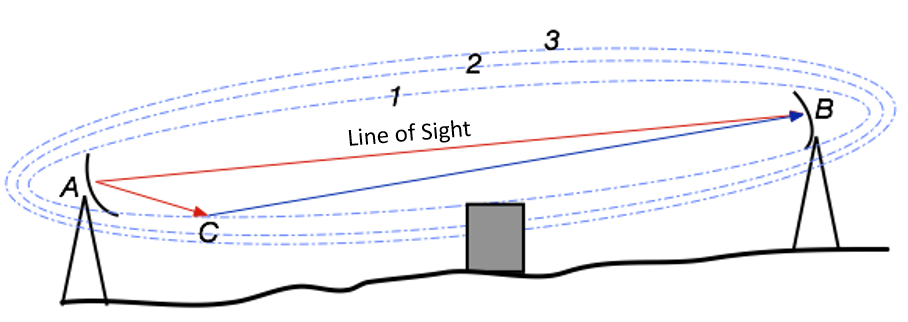
\includegraphics[scale=0.65]{figures/fresnel_zones.png}
	\caption{Fresnel zones between transmitter and receiver}
	\label{fig:fresnel_zones}
\end{figure}

On the figure three Fresnel zones are shown, but there is an infinite number of Fresnel Zones and the 1st Fresnel Zone is the one that has most effect on the performance of the Wireless Network. If there are any obstructions, such as buildings, trees or hills, located in the 1st Fresnel Zone, the signal will be affected by these and would therefore be weakened at the receiver.

Therefore it is a good idea when planning wireless links to keep the 1st Fresnel Zone clear of obstruction. But this can be impractical so it is said that at least 60 $\%$ of the signal should be clear of obstructions. But to get optimum performance it is recommended to keep the signal 20$\%$ or less blocked. \\
%Note that obstacles in the 1st Fresnel Zone will create signals that will be 0 to 90 degrees out of phase, 90 to 270 degrees out of phase in the second zone, 270 to 450 degrees out of phase in third zone and so on.
%
%The first Fresnel zone is the ellipse with chords 1/2 wavelength longer than the direct path (ACB). 
%
%A clear line of sight is needed to maintain signal strength.%Especially for 2.4GHz wireless sytems. This is because 2.4GHz waves are absorbed by water, like the water found in trees. \hl{need something here}
%
%The direct wave, Line of Sight, goes directly from A to B and in this example it is where nothing is blocking the signal. 
%
\subsection{Calculating the Fresnel Zones}
To calculate the Fresnel zone radius at any point P in between the endpoints of the link is given by the following equation: 

\begin{align}
F_n = \sqrt{\frac{n \lambda d_1 d_2}{d_1+d_2}} \label{fresnel_zone_cal}
\end{align}

Where:
\begin{itemize}[label=]
\item $F_n$ = The nth Fresnel Zone radius in metres
\item d1 = The distance of P from one end in metres
\item d2 = The distance of P from the other end in metres
\item $\lambda$ = The wavelength of the transmitted signal in metres
\end{itemize}

\noindent On figure \ref{fig:fresnel_zones} the parameters from equation \ref{fresnel_zone_cal} is shown. 
\begin{figure}[H]
	\centering
	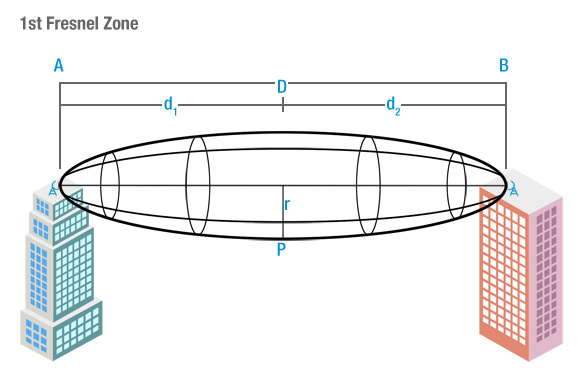
\includegraphics[scale=0.70]{figures/fresnel_zone.jpg}
	\caption{Fresnel zones}
	\label{fig:fresnel_zones}
\end{figure}  

\subsection{Calculating the 1st Fresnel Zone}
Since the 1st Fresnel Zone is the most important, it is often useful to know the maximum radius of the zone. Therefore the following equation will calculate this: (\hl{Maybe show how we come from} \ref{fresnel_zone_cal} to \ref{eq:fresnel_radius} \hl{? - Kelvin})

\begin{align}
r= 8.657 \sqrt{\frac{D}{f}} \label{eq:fresnel_radius}
\end{align}

Where:
\begin{itemize}[label=]
    \item $r$: radius in metres
    \item $D$: total distance in kilometres
    \item $f$: frequency at which are transmitted in gigahertz
\end{itemize}

\noindent In equation \ref{eq:fresnel_radius} it is clear that by changing the distance between the antennas, the radius of the Fresnel zone will also change. To show how the radius changes by changing the distance, some examples are made. In these examples a frequency of 2.4Ghz are used. The first example shows an antenna in the height of 20 meter and a drone flying in the height of 100 meter with 10km between them.

\begin{figure}[H]
	\centering
	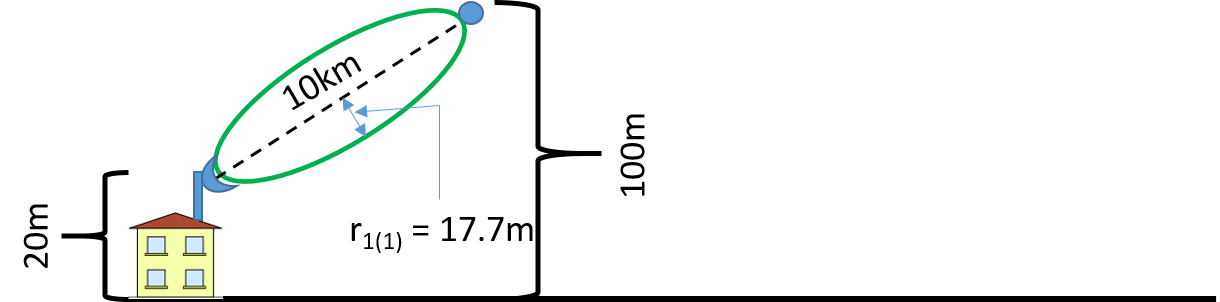
\includegraphics[scale=0.50]{figures/fresnel_10km.png}
	\caption{Fresnel zones between transmitter and receiver 10km}
	\label{fig:fresnel_zones_10km}
\end{figure}  

And the radius calculated:
\begin{align*}
r1 = 8.657\cdot \sqrt{\frac{10}{2.4}} = 17.7m
\end{align*}

The second example are with a distance between them of 20km:

\begin{figure}[H]
	\centering
	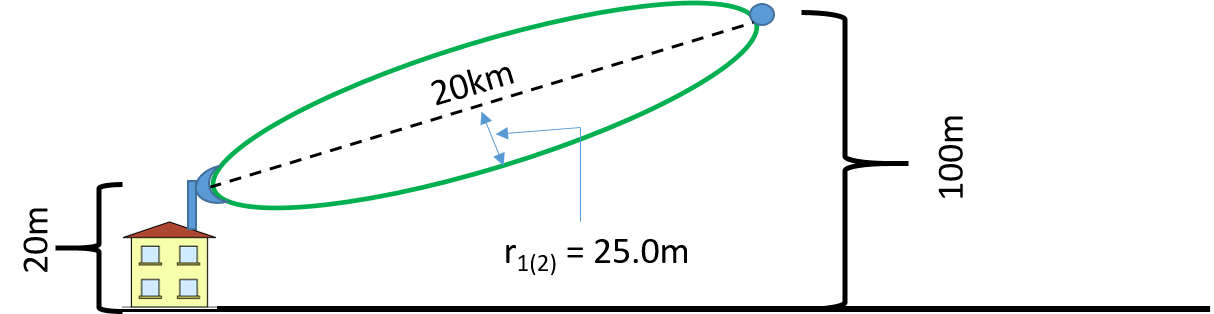
\includegraphics[scale=0.50]{figures/fresnel_20km.png}
	\caption{Fresnel zones between transmitter and receiver 20km}
	\label{fig:fresnel_zones_20km}
\end{figure}  

And the radius calculated:
\begin{align*}
r2 = 8.657\cdot \sqrt{\frac{20}{2.4}} = 25.0m
\end{align*}

The third example are with a distance between them of 20km:

\begin{figure}[H]
	\centering
	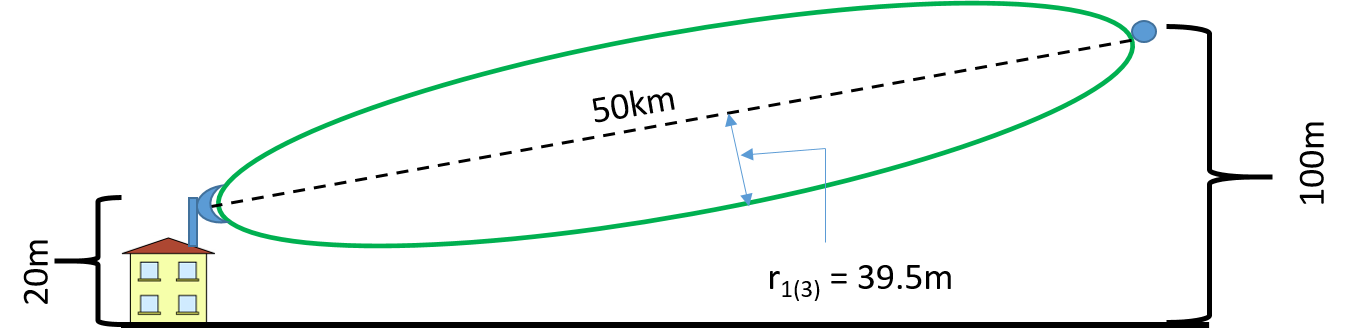
\includegraphics[scale=0.50]{figures/fresnel_50km.png}
	\caption{Fresnel zones between transmitter and receiver 50km}
	\label{fig:fresnel_zones_50km}
\end{figure}  

And the radius calculated:
\begin{align*}
r3 = 8.657\cdot \sqrt{\frac{50}{2.4}} = 39.5m
\end{align*}

\noindent In these examples it is demonstrated that the radius of the Fresnel Zone increases when the distance between the antennas increases.
\newpage
%The 1st zone is the ellipse with chords 1/2 wavelength longer than the direct path (ACB).
%If a reflective object is very near the direct path, the signal will experience a 180o phase shift and cancel the direct wave at the receiver.
%If a reflective object is tangent to the 1st zone, the electromagnetic wave will be shifted 180o because of the increased path length, undergo an additional 180o phase shift due to the reflection, and reinforce the direct wave at the receiver. Consequently, there should be no reflective objects in the 1st Fresnel zone.
%If unobstructed, radio waves will travel in a straight line from the transmitter to the receiver. But if there are reflective surfaces along the path, such as bodies of water or smooth terrain, the radio waves reflecting off those surfaces may arrive either out of phase or in phase with the signals that travel directly to the receiver. Waves that reflect off of surfaces within an even Fresnel zone are out of phase with the direct-path wave and reduce the power of the received signal. Waves that reflect off of surfaces within an odd Fresnel zone are in phase with the direct-path wave and can enhance the power of the received signal. Sometimes this results in the counter-intuitive finding that reducing the height of an antenna increases the signal-to-noise ratio.
%Fresnel provided a means to calculate where the zones are—where a given obstacle will cause mostly in phase or mostly out of phase reflections between the transmitter and the receiver. Obstacles in the first Fresnel zone will create signals with a path-length phase shift of 0 to 180 degrees, in the second zone they will be 180 to 360 degrees out of phase, and so on. Even numbered zones have the maximum phase cancelling effect and odd numbered zones may actually add to the signal power.[1]
%To maximize receiver strength, one needs to minimize the effect of obstruction loss by removing obstacles from the radio frequency line of sight (RF LoS). The strongest signals are on the direct line between transmitter and receiver and always lie in the first Fresnel zone.
